\chapter{Characterization of CUDA kernels}\label{chap:characterization}
\section{Introduction}
\label{sec:IntroGPU}
\lettrine[findent=2pt]{\textbf{G}}{}PUs initially had only graphical function, but their potential as co-processors and accelerators was quickly perceived and new computing platforms evolved to support and take advance of these devices. Different industries, e.g, video games, design 3D, image rendering and computer simulation required more computational features and, as a result of this need, new GPU architectures became more flexible and powerful. Nowadays, we can find on the market, GPUs with thousands of processors for general purpose computing that are used in numerous and different fields. 

The two major GPU manufacturers today are NVIDIA and AMD, which produce GPUs that operate in conjunction with standard CPUs. The main programming environments for GPUs are CUDA~\citep{CUDAGuide} and OpenCL~\citep{khronos:opencl}. OpenCL is considerably more recent than CUDA. One of the main dilemma of OpenCL is to maintain performance while preserving portability between distinct devices~\citep{Du2012391}. 
%The most widely used GPUs are those produced by NVIDIA, together with the CUDA platform. Considering that the GPGPU market has been taken by NVIDIA graphics cards, our models and experimentation are done on GPUs manufactured by NVIDIA.

%The architecture of these GPUs is built with a set of Streaming Multiprocessors (SMs), each containing several cores called Scalar Processors (SPs), a set of Special Function Units (SFUs) and a number of load/store units. The multiprocessors execute asynchronously, in parallel. The SM schedules threads in groups of 32 parallel threads called warps, which can use load/store units concurrently, allowing simultaneous reads from memory for these threads. 

This chapter is organized in four sections, Section~\ref{sec:GPUsCUDA} discuss relevant advances in GPU architectures and their development platform CUDA, Section~\ref{sec:methodChar} shows the GPU test bed and the different benchmark that were selected in order to perform our experiments. Finally, Section~\ref{sec:commOpt} shows the main communication optimizations of CUDA applications and other different optimization to be performed by CUDA applications
%  we explain how different streams work in a GPU in Section~\ref{sec:StreamGPU}.

\section{GPU Architectures and CUDA}\label{sec:GPUsCUDA}
The most widely GPUs used for High Performance Computing are those produced by NVIDIA. The architecture of these GPUs is based on a set of Streaming Multiprocessors (SMs), each containing Streaming Processors (SPs), a set of Special Function Units (SFUs) and a number of load/store (LD/ST) units. The multiprocessors execute threads asynchronously, in parallel. The SM schedules threads in groups of 32 parallel threads called warps, which can use LD/ST units concurrently, allowing simultaneous reads and writes to memory. Above the main parts of a GPU is explained:

\begin{itemize}
    \item Graphic Processing Clusters (GPC): TPC is a chip which grouped the streaming multiprocessor in a GPU. Single GPC contains a raster engine. It is a way to encapsulate all key graphics processing units. Before to Fermi, SMs and Texture Units were grouped together in hardware blocks called Texture Processing Clusters (TPCs). But after Fermi, SMs have dedicated Texture Units. 
    
    \item Streaming Multiprocessors (SM): A SM is designed to execute thousands of threads concurrently, up to 2048 threads on recent architectures. To manage such a large amount of threads, the instructions are pipelined through simultaneous hardware multithreading. These hardware units are SP, SFU, LD/ST, among others. The smallest executable unit of parallelism on a NVIDIA device is 32 threads or a warp. Normally different architectures have a different number of SMs and the number of hardware units inside it. 
    
    \item Hardware units: Streaming multiprocessor are commonly organized by FP32 and FP64 cores, SFU and LD/ST units. FP32 and FP64 cores are shaders processors which are designed to do streaming floating point calculations. SFUs are special function unit for "fast approximate transcendental operations". They execute transcendental instructions such as \textit{sin}, \textit{cosine} and \textit{square root}, with each SFU executing one instruction per clock. Load/Store units are used to read and write in the global memory. One instruction can read/write up to 128 bytes, as a consequence, if each thread in a warp reads 4 bytes and they are coalesced, then whole warp would require a single load/store instruction. If accesses are uncoalesced, then more transaction should be issued.
    
\end{itemize}

Until now, the GPU architectures manufactured by NVIDIA are Tesla, Fermi, Kepler, Maxwell, Pascal and recently Volta. Generally, the hierarchical memory of a NVIDIA GPU contains global and shared portions. Global memory is large, an off-chip, has a high latency and can be accessed by all threads in the GPU. Shared memory is small, on-chip on each SM, has a low-latency and can be accessed only by threads in the same SM. Each SM has its own shared L1 cache and an off-chip coherent global L2 cache. 

All NVIDIA architectures vary in a large number of features, such as the number of cores, registers, SFUs, load/store (LD/ST) units, cache memory sizes, processor clock frequency, memory bandwidth, unified virtual memory, and dynamic parallelism. One main challenge in the designing of new generations of massively parallel architectures is the ratio of improvement between energy consumption and performance~\citep{Mittal:2014}. 
Those differences are summarized in the Compute Capability (C.C.) of NVIDIA GPUs, shown in Table~\ref{tab:CC}. Many of these differences will be exposed in Subsection \ref{ssec:GPUroadmap}, where we mention some technical specifications of each NVIDIA GPU architecture.  

\subsection{NVIDIA GPU Roadmap}\label{ssec:GPUroadmap}

\paragraph{Tesla Architecture:}
This architecture was one of the first GPU to support C or CUDA, allowing programmers to use these devices without having to learn a new programming language. 
Currently, Tesla is also the name of the GPUs designed for High Performance Computing. 

The model GeForce 8800 was one of the first model designed with this architecture, see Figure~\ref{fig:GTX:8800}. This GPU has 112 SP, these SPs were grouped in seven independent chips called Texture/Processor Clusters (TPCs)~\citep{2008:TeslaGPU}. Each TPC has 2 SM and each SM consists of eight streaming processors, 16KB of on-chip shared memory, two SFUs, a constant cache, a multithreaded instruction fetch and issue unit and a read-only constant cache. Second versions of Tesla architectures implemented fused multiply-add (FMA) for double precision.

\begin{figure}[htpb]
\centering
\includegraphics[scale=.85]{images/GeForce-8800-GTX-2-1.png}
\caption{GPU GeForce GTX 8800, the first to support CUDA platform, extracted  from NVIDIA Documentation}
\label{fig:GTX:8800}
\end{figure}

\paragraph{Fermi Architecture:} Fermi architectures implemented the IEEE 754-2008 floating-point standard \citep{FMA-IEEE} for both single and double precision arithmetic which performs multiplication and addition with a single rounding step. In this architecture is possible to have a second-level cache L2 shared by all SMs and each SM has a memory cache L1.

A NVIDIA's Fermi GF-100 has 4 GPC, each GPC has 4 SMs for a total of 16 Streaming Multiprocessors. Each SM is composed of 32 cores, resulting in a total of 512 cores. It also has 4 SFUs, 2 warp schedulers, and 16 LD/ST units. Now it has configurable cache L1 or shared memory of 64KB, these configurations can be of 48 KB of shared memory and 16 KB of L1 cache or 16 KB of shared memory and 48KB of L1 cache. 

Among the most important characteristics of programmability of this architecture were to allow concurrent kernel execution, out of order thread block executions and dual overlapped memory transfer engines.

\paragraph{Kepler Architecture:}
In this architecture, the abbreviation for SM changed to SMX. Each SMX has 4 warp schedulers and eight instruction dispatch units, allowing four warps to be issued and executed concurrently. Unlike Fermi, Kepler architectures allow double precision instructions to be paired with other instructions. The shared memory continues sharing the same chip than L1 cache and the same size, 64KB, but now this architecture allowed the configuration of the shared memory and cache memory L1 in different 3 sizes. The 3 different configurations in KB for shared memory and L1 cache are 48/16 32/32 or 16/48. Kepler also introduced a 48KB of cache for read‐only data for SM. 

The GeForce GTX 680 GPU consists of four GPCs, each one of 4 SM for a total of 16 Streaming Multiprocessors. Each SM is composed of 192 cores, resulting in a total of 1536 cores. It has also 32 SFU, 4 warp scheduler and 32 LD/ST units. 

Among the most important characteristics of programmability of this architecture were the addition of dynamic parallelism and hyper-Q. Dynamic Parallelism allowed the GPU to create new work for itself, synchronize on results, and control the scheduling without involving the CPU. Hyper-Q enables different host threads to trigger execution of kernels simultaneously, in the Kepler architecture 32 concurrent connections are possible with the CPU. 


\paragraph{Maxwell Architecture:} 
The L1 cache is shared now with the texture cache with a size of 24 Kb. Unlike in Kepler and Fermi, the Maxwell architecture has a dedicated shared memory and does not share level with the level 1 cache. The shared memory now is a dedicated chip of 96 KB. Scheduling algorithms have been rewritten to avoid stalls\footnote{stalls is a delay before the processor can continue to execute a statement}, thus reducing the amount of energy spent per instruction. 

GPU Maxwell GM204 consists of four GPCs, each one of 4 SM for a total of 16 Streaming Processors. Each SM is composed of 128  cores, resulting in a total of 2048 CUDA cores. This time, the SMs are partitioned into 4 blocks, each with its instruction buffer, its scheduler. Each block also has 8 LD/ST units, 8 SFU. 
The main features introduced by the Maxwell architecture are related to power consumption and Unified Virtual Addressing (UVA). UVA allows direct access between the host and the devices, without requiring a buffer in the host to perform data transfer.

\paragraph{Pascal Architecture:}
Pascal architecture brings big changes in NVIDIA GPUs, it introduces the new technology of stacked DRAM memory and it brings a new technology of interconnection between GPUs named NVlink. Another important characteristic of this architecture is the addition of preemption, now GPU applications are available to do preemption during their executions. 

Pascal continues which the groups of multiprocessors in GPC and the dedicated chip for shared memory per Streaming Multiprocessors. Cache L1 continues sharing the same chip than Texture cache, but the size increased to 48KB.

\paragraph{Volta Architecture:} This architecture has came optimized for Deep Learning applications. Save energy has been an important parameter in the design of this architecture, in comparison with Pascal GPUs the new Volta SM is 50\% more energy efficient than the previous Pascal architecture. This architecture introduces a new characteristic, this characteristic is named \textbf{Tensor Cores}. Shared memory back to be combined with a L1 cache memory. This chip-on memory increased its size and it is now of 124 MB and shared memory is configurable up to 96 KB.

A Volta GV-100 has 6 GPC, each GPC inside has 14 SMs and each SM has 64 SP for a total of 5376 cores. The GV100 SM is partitioned into four processing blocks, each with 16 FP32 units, 8 FP64 units, two tensor cores for deep learning matrix arithmetic, one warp scheduler and one dispatch unit. 

One of the main characteristics in the programmability is the concept of Cooperative Groups, the is a new programming model for organizing groups of communicating threads, it allows developers to express the granularity at which threads are communicating. Table~\ref{tab:CC} shows a better summary of the main Tesla GPU architectures manufactured by NVIDIA.


\begin{table}[htpb]
    \centering
    \begin{tabular}{|r|c|c|c|c|c|}
    \hline\hline
        {\bf Features/Teslas}&{\bf Fermi}&{\bf Kepler}&{\bf Maxwell}&{\bf Pascal}&{\bf Volta}\\\hline
        % Features&Fermi GF100&Kepler GK110&Maxwell GM200&Pascal GP100\\\hline
         Compute Capability&2.0&3.5&5.3&6.0&7.0\\\hline
        %  SMs per GPCs&1&1&4&10&14\\\hline
         SMs &13&15&24&56&84\\\hline
         SPs per SM &32&192&128&64&64\\\hline
         FP32 Units&512&2880&3072&3840&5376\\\hline
         FP64 Units &-&512&960&1792&2560\\\hline
        %  FP64 Units &-&512&960&1792&2560\\\hline
        %  Memory Interface&384-bit GDDR5&384-bit GDDR5&384-bit GDDR5&4096-bit HBM2&4096-bit HBM2\\\hline
         Max Warps per SM&48&64&64&64&64\\\hline
         Max Thread per SM&1536&2048&2048&2048&2048\\\hline
         Shared memory size (KB)&48&48&96&64&up to 96\\\hline
         Manufacturing process (nm)&40&28&28&16FinFET&12 FinFET\\\hline
         Hyper-Q&No&Yes&Yes&Yes&Yes\\\hline
         Dynamic Parallelism&No&Yes&Yes&Yes&Yes\\\hline
         Unified Memory&No&No&No&Yes&Yes\\\hline
         Preemption&No&No&No&Yes&Yes\\\hline\hline
          
    \end{tabular}
    \caption{Description of the Compute Capability of the last GPU NVIDIA architectures}
    \label{tab:CC}
\end{table}

On the left side of Figure~\ref{fig:hierarchyThread} is shown the memory hierarchy of a thread that runs on a GPU with Fermi architecture. In this architecture, the L1 cache is in the same chip than shared memory. On the middle is shown the memory hierarchy of a thread that runs on a GPU with Kepler or Volta architecture, in this architecture a cache read-only is added and the L1 cache is in the same chip than Shared memory. In the right side is shown a memory hierarchy of a thread which runs on a GPU with Maxwell or Pascal architecture, in these architectures the shared memory is dedicated and the L1 cache is in the same chip than a texture cache. Figures were modified from the NVIDIA documentation.

\begin{figure}[htpb]
\centering
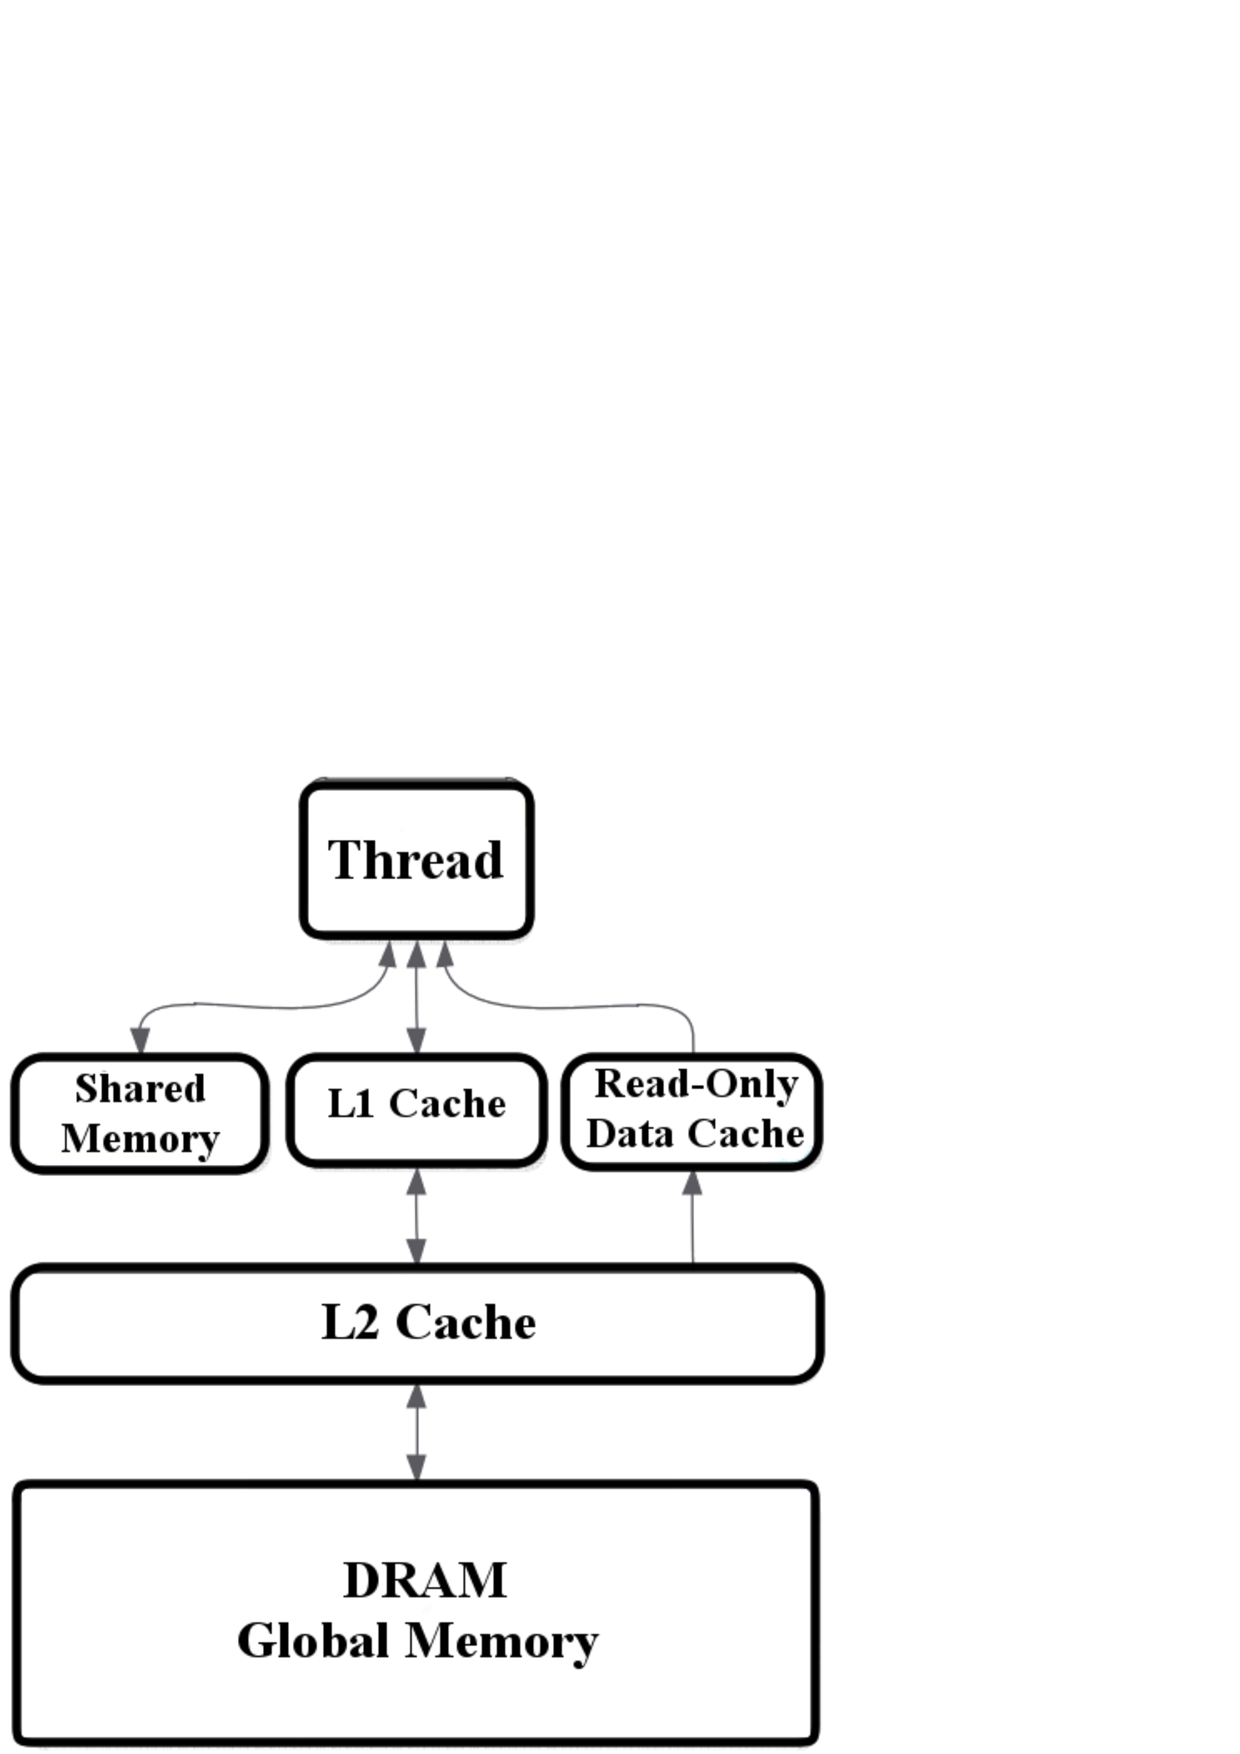
\includegraphics[scale=.25]{./images/hierarchyThread.png}
\caption{Left: Memory hierarchy accessed from a thread in a GPU with Fermi architecture. Right: Memory hierarchy accessed from a thread in a GPU with Kepler architecture}
\label{fig:hierarchyThread}
\end{figure}

\subsection{\textit{Compute Unified Device Architecture} (CUDA)}\label{ssec:CUDA}
The parallelism reached by the GPUs of NVIDIA is of the type Single Instruction Multiple Data (SIMD), but commonly NVIDIA denominates this type of parallelism \emph{Single Instruction Multiple Threads} (SIMT), where thousands or millions of threads are executed concurrently into the GPU. In the type of parallelism used by the SIMT, an application launches a function with many threads which will execute the same instructions, and threads are programmed dynamically in a SIMD-like parallelism to access data.  By itself, SIMD only describes how the instructions are executed. 

The SIMT programming model has an approach that is different from the traditional \textit{multicore} processor model. In particular, the Open Computing Language (OpenCL) is a low-level API for writing programs that can execute across heterogeneous computing systems (i.e., consisting of GPUs and CPUs) and even other kinds of processing units. CUDA and others tools provide ways to parallel computing using data-based or task-based parallelism on different architectures. CUDA works in a single-instruction multiple-data parallelism, where data is accessed by the index of each thread in a CUDA function.

The CUDA platform enables the use of NVIDIA GPUs for scientific and general purpose computation. A single \textit{master} thread runs in the CPU, launching and managing computations on the GPU. GPUs have their own memory and data must be transferred through a PCI Express bus. Data for the computations have to be transferred from the host memory to the device memory. Actually, the execution flow of a GPU application can be divided into three key stages. First, data is transferred to the memory of the GPU; in a second stage, the main program executed on the CPU (called host) is responsible for starting threads in the GPU (called device), launching a function (called kernel). Finally, results are sent back to the host. Figure~\ref{fig:cuda:model} shows a classical execution workflow of a CUDA application.

\begin {figure}[htpb]
  \centering
  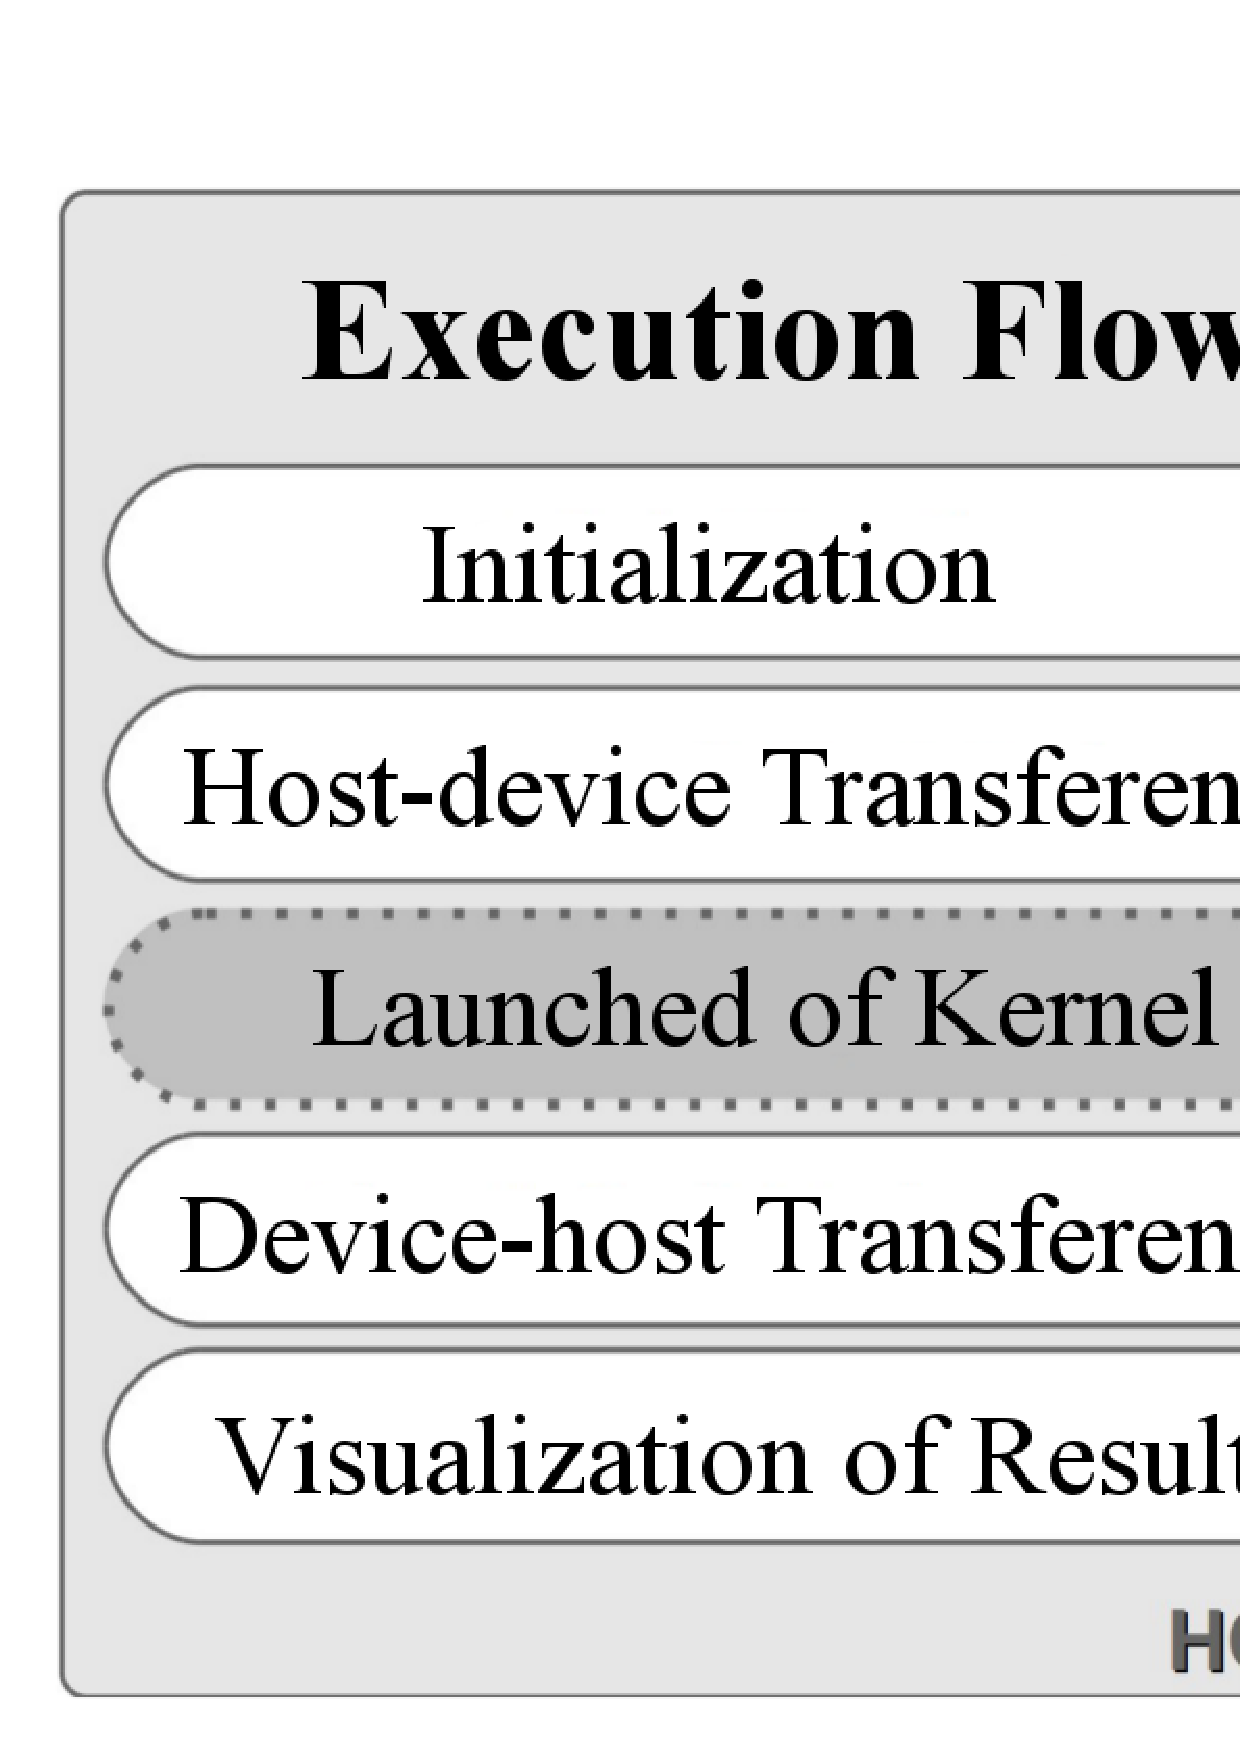
\includegraphics[width =.45\textwidth] {images/modelo-classico-execucao.png}
  \caption{Classical Execution of a GPU application}
  \label{fig:cuda:model}
\end {figure}

The CUDA language extends C and provides a multi-step compiler, called \texttt{NVCC}, that translates CUDA code to Parallel Thread Execution code or \emph{PTX}. \texttt{NVCC} uses the host's C++ compiler in several compilation steps, and also to generate code to be executed in the host. The final binary generated by \texttt{NVCC} contains code for the GPU and the host. When \texttt{PTX} code is loaded by an application at run-time, it is compiled to binary code by the host's device driver. This binary code can be executed in the device's processing cores and is architecture-specific. The targeted architecture can be specified using \texttt{NVCC} parameters~\citep{CUDAGuide}. 

When a kernel is launched, $t$ parallel threads are executed into the CUDA cores of a GPU. All threads execute a copy of the same code defined in the body declaration of the kernel function. The number of threads in a kernel is defined in two tri-dimensional parameters. The number of threads in a block and the number of blocks in a grid, the special words in CUDA to define those parameters are \texttt{blockDim} and \texttt{gridDim}, respectively. Each kernel create a grid of threads into the GPU, each grid is organized by blocks and these blocks are divided by threads, see Figure~\ref{fig:dimGridBlock}. It is normal to associate the dimension of the block to the dimension of the problem to solve.

\begin{figure}[htpb]
    \centering
    \includegraphics[scale=.85]{images/Kernel-grid-organization.png}
\caption{Thread hierarchy and memory visibility of a kernel, copied from NVIDIA Documentation}
\label{fig:dimGridBlock}
\end{figure}

Threads in a grid have access to different memory types. Threads in the same block can access with a high bandwidth to registers, shared memory and local memory, i.e. on-chip memory in the SM. All threads in the grid have access to load and write in the global, but only to load from the constant and texture memory, see Figure~\ref{fig:dimGridBlock}. Threads can be synchronized on two different levels, global memory, and shared memory. Thread into the same block can be synchronized across the shared memory with a high bandwidth. All threads in a kernel are synchronized across the global memory with a bandwidth lesser than shared memory, resulting in an expensive instruction for GPU applications.

The maximum number of threads in a block or blocks in a grid is specific for each compute capability, these values are shown in Table~\ref{tab:CC}. something to notice In this table is the number of SPs per SM which increase in the Kepler architecture and after decreases in the next architectures; and the number maximum of warp per SM increase in Kepler and it keeps  the same (64) in posterior architectures. This ensures a better occupancy of the SM.

If threads of the same warp execute different instructions, i.e. warps executing a conditional statement, the CUDA compiler must generate code to branch the execution correctly, making the program lose performance due to this \emph{warp divergence}. Code divergence greatly degrades the performance of an application running on such architectures. 

The bandwidth of the global memory can be largely improved by combining the LD/ST requests from different threads of a single warp, in a process called coalescing~\citep{confwdagHaTA08}. The coalescing occurs when the threads access contiguous global memory addresses, which permits usage of the multiple LD/ST units available per SM.% All the levels of the memory hierarchy are benefited by this communication optimization.

Multiple computations launched by the master thread, or \textit{kernels}, can run asynchronously and concurrently in a current GPU. In CUDA, all kernel executions are asynchronous, threads of the same block can be synchronized with the function \texttt{{\_\_}syncthreads()} and the function \texttt{cudaThreadSynchonize()} can synchronize all the threads of a kernel or grid. 

Finally, all threads of a grid are mapped, and receive identifiers corresponding to the declared dimensions. These identifiers
are available and accessible in CUDA code through variables such as \texttt{threadIdx} and \texttt{blockIdx}. This allows the execution, identification and control of threads in a GPU. The identifiers \texttt{threadIdx.x}, \texttt{threadIdx.y} and \texttt{threadIdx.z} are associated with the threads within a block and \texttt{blockIdx.x}, \texttt{blockIdx.y} and \texttt{blockIdx.z} are associated with the index of a block within a grid.

In the next section, we describe each one of the kernels used as benchmarks in this research and discuss main characteristics of communication and computation of each one. 


%=================================================================
\section{GPU Testbed and Selected CUDA kernels} \label{sec:methodChar}
Several different benchmarks have been proposed in the literature to measure and assess existing GPGPU heterogeneous architectures, such as Rodinia~\citep{Rodinia:Che:2009}, Parboil~\citep{Stratton:2012:Parboil} and SHOC~\citep{Danalis:2010:SHOC}. Rodinia benchmark was devised for heterogeneous parallel computing research, it has had a high level of acceptance in the community and its applications represent different high-level domains or behaviours,  called the Berkeley dwarfs~\cite{asanovic2009dwarfs}. In this work, we have selected  a set of GPU Applications from the Rodinia Benchmark suite and  other classical algorithms of linear algebra. First to all, we present in the next subsection the different GPUs that we used for our experiments. After in Subsection~\ref{ssec:useCases}, we characterize each one of the kernel that we used for our experiments.

%For each application we iterated over the values of one or two parameters, with some applications invoking the same kernel multiple times on each execution. During our evaluation, all applications were executed using the CUDA profiling tool \textit{nvprof}. Each experiment is presented as the average of ten executions, with a confidence interval of 95\%. In this section we describe the GPU applications, GPU testbed used to do this work.

%---------------------------------------------------------------------------

\subsection{GPU Testbed}\label{ssec:GPUTestbed}
For our experiments in the Chapter~\ref{chap:BSPmodel} and Chapter~\ref{Chap:ML} we used 9 different GPUs, described in Table~\ref{tab:GPUs}, with 5 belonging to Kepler architecture (Compute Capability 3.X), 3 to Maxwell (C.C. 5.X) and 1 to Pascal (C.C. 6.x). More information about these GPUs are presented in Table~\ref{tab:CC} and we have described the main changes of hardware and software between architectures in Section~\ref{ssec:GPUroadmap}. 

%Experiments with the Tesla Pascal P-100 were performed accessing the Free OpenPOWER Cloud by Unicamp, running in an IBM OpenPOWER Server configured with 16 physical cores, up to 128 simultaneous treads or vcpus, and 2 x NVIDIA GPU Tesla-P100, connected via NVLINK 1.0. 

% \todoRaph{You described where the Pascal experiments were performed. And the other boards? \textbf{Corrected - That was question of acknowledge}}

\begin{table}[htpb]
    \centering
    \scalebox{0.75}{
    \begin{tabular}{lccccccc}
        \toprule
        \textbf{Model}&\textbf{C.C.}&\textbf{Memory}&\textbf{Bus}&\textbf{Bandwidth}&\textbf{L2}&\textbf{Cores/SM}&\textbf{Clock} \\ \bottomrule
        GTX-680&3.0&2 GB&256-bit&192.2 GB/s&0.5 M&1536/8&1058 Mhz \\ \midrule 
        Tesla-K40&3.5&12 GB&384-bit&276.5 GB/s&1.5 MB&2880/15&745 Mhz \\ \midrule
        Tesla-K20&3.5&4 GB&320-bit&200 GB/s&1 MB&2496/13&706 MHz\\ \midrule
        %Titan Black&3.5&6 GB&384-bit&336 GB/s&1.5 MB&2880/15 &980 Mhz \\ \midrule
        Titan&3.5&6 GB&384-bit&288.4 GB/s&1.5 MB&2688/14&876 Mhz\\ \midrule
        Quadro K5200&3.5&8 GB&256-bit&192.2 Gb/s&1 MB&2304/12&771 Mhz \\ \midrule
        Titan X&5.2&12 GB&384-bit&336.5 GB/s&3 MB&3072/24&1076 Mhz \\ \midrule
        GTX-970&5.2&4 GB&256-bit&224.3 GB/s&1.75 MB&1664/13&1279 Mhz\\ \midrule
        GTX-980&5.2&4 GB&256-bit&224.3 GB/s&2 MB&2048/16&1216 Mhz \\ \midrule
        Pascal-P100&6.0 GB&16 GB&4096-bit&732 GB/s&4 MB&3584/56&1328 Mhz\\ \midrule
    \end{tabular}}
    \caption{Hardware specifications of the GPUs in the testbed}
    \label{tab:GPUs}
\end{table}

\subsection{Selected CUDA kernels}\label{ssec:useCases}
The  source code for all the use cases, experiments and results are available\footnote{Hosted at GitHub: \texttt{\scriptsize https://github.com/marcosamaris/gpuperfpredict} [Accessed on March 2018]} under Creative Commons Public License for the sake of reproducibility. 

Our benchmark contains 4 different strategies for \emph{matrix multiplication}~\citep{CUDAGuide}, 2 algorithms for \emph{matrix addition}, 1 dot product algorithm, 1 vector addition algorithm and 1 \emph{maximum sub-array problem} algorithm~\citep{Cleber:Thesis}, and 11 CUDA kernel functions belonging to 6 applications from Rodinia benchmarking suite (see Table~\ref{tab:Rodinia}). The remainder of this section discusses some details of these algorithms, and introduces a code of letters for each application, used in Chapter~\ref{chap:BSPmodel} and Chapter~\ref{Chap:ML}.

\subsubsection{Matrix Multiplication}
Matrix multiplication is the core of many scientific areas. This operation is highly used in areas like deep learning, visual computing and digital images processing, among others. The analysis and modeling of these algorithms brings a better understanding and help to researcher and developer of Job Management Systems to deal with this mathematical operations.

In this research, we used four different versions of matrix multiplication, these versions differ in memory access optimizations: global memory with non-coalesced accesses (MMGU); global memory with coalesced accesses (MMGC); shared memory with non-coalesced accesses (MMSU); and shared memory with coalesced accesses (MMSC). This algorithm has a high utilization of the Streaming Processors and it obtains a high throughput of communication in the different levels of memory, L2 cache and L1 cache for small matrices. We have adopted \texttt{block\_size}$^2$ threads per block and defined the number of blocks to be square of \texttt{(N + block\_size-1)/block\_size}, dynamically devised from the size of the problem ($N$) and the block size. Aiming to take advance of coalesced accesses the value of \texttt{block\_size} is equal to 16 in our experiments. In Section~\ref{sec:characterization} is presented an communication analysis of this application with different sizes of threads per block.

The asymptotic computational complexity of a square matrix multiplication of size $N$ is $O(N^3)$ in a sequential algorithm, in a CUDA algorithm this complexity is $O(N)$ using $N\times{}N$ threads. In this algorithm each thread requests $N$ elements from both matrices and perform a dot product with these arrays. This CUDA kernel performs $N$ reads from global memory for each matrix and $N$ arithmetic operations. A single write instruction is performed. shared memory is not used in two versions, MMGU and MMGC. In Figure~\ref{fig:matMulGMUN} is shown the source code of the kernel MMGU, we only changed the data access pattern, to permit coalesced accesses to data in global memory. In Figure \ref{fig:matMulGMUN} line 7 is changed to \texttt{Pvalue += A\_d[i * N + k] * B\_d[k * N + j];} and line 10 is changed to \texttt{C\_d[i * Width + j] = Pvalue;}.

\lstset{emph={[2]__global__}, emphstyle={[2]\color{red}\bf },language=C++, keywordstyle=\color{blue}, numbers=left, showspaces=false,
    showstringspaces=false, tabsize=1, breaklines=false,stringstyle=\color{red}, commentstyle=\color{red}, morecomment=[l][\color{magenta}]{\#}}

\begin{figure}[htpb]
\centering
{\scriptsize
\begin{lstlisting}
__global__ void matMul(float* C_d, float* A_d, float* B_d, int N) {
  float Pvalue = 0.0;
  int j = blockIdx.x * blockDim.x + threadIdx.x;
  int i = blockIdx.y * blockDim.y + threadIdx.y;

  for (int k = 0; k < N; ++k) 
    Pvalue += A_d[j * N + k] * B_d[k * N + i];
  
  C_d[j * N + i] = Pvalue;
}

\end{lstlisting}}
\caption{Kernel in CUDA of matrix multiplication only with global memory and uncoalesced accesses (MMGU).}
\label{fig:matMulGMUN}
\end{figure}

The version MMSU and MMSC use shared memory to load data from global memory and to process them with a lower latency of communication. As shared memory is limited in GPU architectures, the implementations of matrix multiplication with shared memory must be tiled. The concept of tiling in shared memory is graphically described with Figure~\ref{fig:TilingMMSU}, with the matrix multiplication. Tiling is a common strategy to partition data into subset called tiles such that each tile fits into the shared memory. This technique splits our problem domain into phases. The tiled process is executed to guarantee that each thread can access data in shared memory to perform its part of the matrix multiplication. 

In process shown in Figure~\ref{fig:TilingMMSU}, a tile process charges a subset from matrix A and Matrix B in the shared memory of the GPU. A barrier synchronization is used to guarantee that all data was loaded in the shared memory, after the calculations are performed, the barrier synchronization guarantees that the shared memory can be safely overwritten. In this application \texttt{tile\_size=block\_size}, consequently the sizes in bytes of both subsets of the matrices will be \texttt{(tile\_size)$^2 \times$FP\_Bytes}, where \texttt{FP\_Bytes} is the size of the single precision used for the application. 

\begin{figure}[htpb]
	\centering
    \includegraphics[scale=.3]{images/square-tiling.png}
    \caption{Tiling technique of the Matrix multiplication using shared memory}
    \label{fig:TilingMMSU}
\end{figure}

\subsubsection{Matrix Addition}
For the Matrix addition algorithm, we used two different memory access optimizations: global memory with non-coalesced accesses (MAU); and global memory with coalesced accesses (MAC);  The run-time complexity for a sequential matrix addition algorithm using two matrices of size $N\times{}N$ is $O(N^2)$. In a CUDA implementation, the run-time complexity of the matrix addition is $O(1)$ using $N^2$ threads. In this algorithm each thread request $1$ element from each one of the matrix elements and perform a single addition. The implementation of this kernel is similar than matrix multiplication. In Figure \ref{fig:matMulGMUN} the loop of the line 6-7 is deleted and the statement with the addition is added \texttt{C[tid] = A[tid] + B[tid];}, where \texttt{tid} = \texttt{int tid = i*N + j;}. To take advances of coalesced accesses, \texttt{tid} is changed to \texttt{int tid = j*N + i;}. 

Matrix addition has the same threads hierarchy than matrix multiplication. The blocks are bi-dimensional with \texttt{block\_size}$^2$ threads per block. The size of the grid is square of \texttt{N/block\_size}, dynamically devised from the size of the problem \texttt{N} and \texttt{block\_size}.

\subsubsection{Vector Addition Algorithm (vAdd)}
For two vectors $A$ and $B$, the Vector Addition $C = A + B$ is obtained by adding the corresponding components. In a CUDA implementation, the run-time complexity of the vector addition algorithm is $O(1)$ using N threads, so each threads perform an addition of a position of the vectors $A$ and $B$ and stores the result in the vector $C$. This algorithm is a simplified version of the matrix addition. This application has an uni-dimensional block, the block size used for the experiments is $256$ and the size of the grid is also uni-dimensional and dynamically devised from the size of the problem  \texttt{N} and \texttt{block\_size}. The source code of this kernel is similar than matrix addition, only change the dimension indexes of each threads, i.e. \texttt{int tid = blockDim.x * blockIdx.x + threadIdx.x;}, using only the dimension $x$ of \texttt{blockDim}.

\subsubsection{Dot Product Algorithm (dotP)}
For two vectors $A$ and $B$, the dot product $C = A \cdot B$ is obtained by adding the multiplication of corresponding components of the input, the result of this operation is a scalar. Unlike vector addition, dot product is a reduction from vectors to a scalar. In a GPU algorithm, each thread performs a multiplication of a position of the vectors $A$ and $B$ and stores the result shared variable. Then a reduction using the shared memory is performed and finally a vector with size equal to \texttt{N/block\_size} is transferred to the CPU memory for later processing. The block size used for the experiments is $256$ and the size of the grid is also uni-dimensional and dynamically devised from the size of the problem  \texttt{N} and \texttt{block\_size}.

\subsubsection{Maximum Sub-Array Problem (MSA)}
Let $X$ be a sequence of $N$ integer numbers $(x_1, ... , x_N)$. The Maximum Sub-Array Problem (MSA) consists of finding the contiguous sub-array within $X$ which has the largest sum of elements. The solution for this problem is frequently used in computational biology for gene identification, analysis of sequence of protein and DNAs, identification of hydrophobic regions, among others. The implementation used in this paper creates a kernel with 4096 threads, divided in 32 blocks with 128 threads~\citep{Cleber:Thesis}. The $N$ elements are divided in intervals of $N/t$, and each block receives a portion of the array. The blocks use the shared memory for storing segments, which are read from the global memory using coalesced accesses. Each interval is reduced to a set of 5 integer variables, which are stored in vector of size $5 \times t$ in global memory. This vector is then transferred to the CPU memory for later processing. 

A summary of each one of these applications is shown in Table~\ref{tab:useCases}, in this table is shown the thread hierarchy and the request shared memory per block in each kernel. In column \texttt{dimGrid} and \texttt{dimBlock} is shown how each solution is associated to the dimension of the problem. Column Shared Mem shows the size of shared memory that each kernel needs per block.

\begin{table}[htpb]
    \centering 
    \scalebox{.9}{
        \begin{tabular}{cccccc} 
            \midrule\midrule
            \textbf{Application} & \textbf{Param} & \textbf{Kernel}& \textbf{\texttt{dimGrid}}&  \textbf{\texttt{dimBlock}}&\textbf{Shared Mem}\\\midrule\midrule   
            \multirow{4}{*}{Matrix Mul} & \multirow{4}{*}{1} &MMGU &\multirow{4}{*}{(GS, GS, 1)}&\multirow{4}{*}{ (BS, BS, 1)}&\multirow{4}{*}{($BS^2\times{}2\times{}4B$)}\\      
            &  &MMGC & & &\\
            &  &MMSU & & &\\   
            &  &MMSC & & &\\\midrule     
            \multirow{2}{*}{Matrix Add} & \multirow{2}{*}{1} &MAU &\multirow{2}{*}{(GS, GS, 1)}&\multirow{2}{*}{ (BS, BS, 1)}&\multirow{2}{*}{0}\\ 
            &  &MAC & & & \\\midrule 
            Vector Add&1  &VAdd &(GS, 1, 1) &(BS, 1, 1)& 0 \\\midrule
            Dot Product&1  &dotP &(GS, 1, 1) &(BS, 1, 1) &($BS\times{}4B$)\\\midrule
            Max. Sub Array&1  &MSA & (48, 1, 1) &(128, 1, 1)&($4096\times{}4B$)\\\midrule
        \end{tabular}}
    \caption{Key linear algebra applications used in the experiments}
    \label{tab:useCases} 
\end{table}

\subsubsection{Rodinia Benchmark Suite}
We selected 11 CUDA kernel functions belonging to 6 applications from Rodinia for the benchmarks (Table~\ref{tab:Rodinia}). Some applications invoke the same kernel multiple times on each execution, resulting in the number of collected samples shown in the last column. For each kernel we iterated over the values of one or two parameters, with the number of iterations indicated inside the brackets. For instance, the Hot Spot application has 2 parameters, with the first iterated among 5 values and the second 4 values, for a total of 20 executions in each machine. %In those applications only some part of them can be compute concurrently, above we will explain the performance behavior of each one of the selected Rodinia benchmarks kernels.

\begin{table*}[htpb]
    \centering 
    \scalebox{.8}{
        \begin{tabular}{cccccc} 
            \midrule\midrule
            \textbf{Application} & \textbf{Berkeley Dwarf} & \textbf{Domain}& \textbf{Param.}& \textbf{Kernels} & \textbf{Samples}\\\midrule\midrule   
            \multirow{2}{*}{Back Propagation (BCK)} & \multirow{2}{*}{Unstructured Grid} & \multirow{2}{*}{Pattern Recognition} &\multirow{2}{*}{1 - [57]}&layerforward&\multirow{2}{*}{57}\\
            &  &  & &adjust-weights  \\\midrule      
            \multirow{2}{*}{Gaussian Elimination (GAU)} & \multirow{2}{*}{Dense Linear Algebra} & \multirow{2}{*}{Linear Algebra} &\multirow{2}{*}{1 - [32]}& Fan1&\multirow{2}{*}{34800}  \\             
            &  &  & & Fan2  \\\midrule
            Heart Wall (HWL) & Structured Grid & Medical Imaging &1 - [84]& heartWall&5270 \\\midrule
            Hot Spot (HOT) & Structured Grid & Physics Simulation &2 - [5,4]& calculate-temp&396288 \\\midrule            
            % Hot Spot 3D (H3D) & Structured Grid & Physics Simulation &2 - [3,10]& hotspotOpt1&150150 \\\midrule                     
            %LavaMD (LMD) & N-Body & Molecular Dynamics &1 - [50]& LavaMD&50\\\midrule
            \multirow{3}{*}{LU Decomposition (LUD)} & \multirow{3}{*}{Dense Linear Algebra} & \multirow{3}{*}{Linear Algebra} &\multirow{3}{*}{1 - [32]}&diagonal&8448 \\
            & & &  & perimeter&8416 \\
        &  &  & & internal&8416 \\\midrule            
            \multirow{2}{*}{Needleman-Wunsch (NDL)} & \multirow{2}{*}{Dynamic Programming} & \multirow{2}{*}{Bioinformatics} &\multirow{2}{*}{2 - [16,10]}& needle-1&21760 \\
             &  &  & & needle-2&21600 \\\midrule
            
        \end{tabular}}
    \caption{Rodinia applications used in the experiments}
    \label{tab:Rodinia} 
\end{table*}

\begin{itemize}
    \item {\bf Back Propagation (BCK):}
BCK trains a layered neural network. The application is comprised of two kernels: Forward Phase (BCK-K1), in which the activation are propagated from the input to the output layer, and Backward Phase (BCK-K2), in which the error between the observed and requested values in the output layer is propagated backwards to adjust the weights and bias values. The time complexity of a back-propagation neural network algorithm on a single processor is of $O(W^3)$; where $W$ is the count of weights in the network. In this CUDA implementation both kernels have a complexity $O(log(BS))$ where $BS=16$. Each block has \texttt{BLOCK\_SIZE}$^2$ number of threads. The number of blocks in the grid is \texttt{(N/block\_size} nad it is dynamically calculated from the layer size ($N$) and the block size.

In kernel (BCK-K1), only one thread (with id 0) in the each block load an element of the input layer on the shared memory, after each thread load an element of the weight matrix on the shared memory. Then, the weight matrix is updated with the values of the input layer. Finally a loop reduction is done with a loop of size log2(block\_size). Inside this loop, log2(block\_size) power instructions are done and log2(block\_size) additions over data in the shared memory. Each interval is reduced to a set of \texttt{grid\_size}$\times$\texttt{block\_size} integer variables. This vector is then transferred to the main memory of the host for later processing. In kernel (BCK-K2), shared memory is not used. According to the source code of (BCK-K2), each thread performs O(1) reads and write in the global memory and does different computations over this data.

\item{\bf Gaussian Elimination (GAU):}
GAU solves a linear system $Ax = b$, the application analyzes an $n\times{}n$ matrix and an associated $1 x n$ vector to solve a 
set of equations with $n$ variables and $n$ unknowns. Gaussian Elimination algorithms has a complexity $O(n^3)$. This application compute the results row by row. The algorithm synchronizes between iterations, but the values calculated in each iteration is computed in parallel, see Figure~\ref{fig:GauCode}.

, where $n$ is the size of the matrix elements in both dimensions, i.e. the matrix is $n\times{}n$. 


The application has two different kernels Fan1 and Fan2, which we call (GAU-K1) and (GAU-K2) respectively. (GAU-1) calculate multiplier matrix and (GAU-2) modify the matrix A into LUD. In the experiments, we varied the size of the matrix. 

In this implementation, First kernel GAU-K1, has a uni-dimensionmal block, each block \texttt{block\_size = 512} threads and the number of block is dynamic and computed with the next expression \texttt{(N/block\_size)}. Second kernel has a bi-dimensional block, its dimension is \texttt{block\_size}$^2$ and \texttt{block\_size = 4} in this implementation. The size of the grid also is dynamic depending to size of the problem $N$and the $BS$ (Block size), and it is computed as \texttt{(N/block\_size)}. Both kernel are iterative, it means that the same kernels are invoked multiple times on a single execution of the whole application. Any of these kernel use the shared memory of the streaming processors. 

\lstset{emph={[2]__global__}, emphstyle={[2]\color{red}\bf },language=C++, keywordstyle=\color{blue}, numbers=left, showspaces=false,
    showstringspaces=false, tabsize=1, breaklines=false,stringstyle=\color{red}, commentstyle=\color{red}, morecomment=[l][\color{magenta}]{\#}}

\begin{figure}[htpb]
\centering
{\scriptsize
\begin{lstlisting}
for (t=0; t<(Size-1); t++) {
		Fan1<<<dimGrid1,dimBlock1>>>(m_cuda,a_cuda,Size,t);
		cudaThreadSynchronize();
		Fan2<<<dimGrid2,dimBlock2>>>(m_cuda,a_cuda,b_cuda,Size,t);
		cudaThreadSynchronize();
	}
\end{lstlisting}}
\caption{Kernel in CUDA of matrix multiplication only with global memory and uncoalesced accesses (MMGU).}
\label{fig:GauCode}
\end{figure}

\item {\bf Heart Wall (HWL):}
HWL tracks the movement of a mouse heart over a sequence of 104 609x590 ultrasound images to record response to the stimulus. In the experiments, we varied the number of frames to process. This kernel has two different stages, in the first stage the kernel performs operations on the first frame to detect initial, partial shapes of inner and outer heart walls in the second stage the kernel presents multiple nested loops that process batches of 10 frames and 51 points in each image. This kernel is very complicated to analyze, i.e. this kernel has 1300 codes lines more or less, it uses 8 variables in the shared memory and 44 variables to store all its computations in each streaming multiprocessor, obtaining a low latency in this process. it runs multiple times depending the number of frame to compute. As the number of threads in a block as the number of blocks in a thread ar uni-dimensionals. For all the experiments, this kernels has a \texttt{block\_size}$= 256$ and a \texttt{grid\_size}$ = 51$. For a total of 13056 threads in each one of the executions. This application modeled a set of  ordinary differential equations (ODEs) that are determined by more than 200 parameters. HWL requires the inclusion of some non-parallel computation into the kernel, leading to a slight warp under-utilization.

% \todoRaph{Describe something about the computations performed in the HWL kernel/application.}

\item {\bf HotSpot (HOT):}
HOT is a tool to estimate processor temperature based on an architectural floor plan and simulated power measurements. This application includes the 2D transient thermal simulation kernel which iteratively solves a series of differential equations to determine block temperatures. This kernel has a bi-dimensional grid and block. The dimension of the block is square of \texttt{block\_size} and \texttt{block\_size}$ = 16$. The size of the grid is the square of \texttt{N/block\_size} and it is dynamic depending the size of the problem and the size of the thread block. In the experiments, we varied two parameters: size of the problem and number of iterations. This application has a single kernel. It uses the shared memory.



\item {\bf LU Decomposition (LUD):}
this is a factorization algoritm, where ''LU'' means \emph{lower upper}, LUD is an algorithm to calculate the solutions of a set of linear equations. The LUD kernel decomposes a matrix as the product of a lower triangular matrix and an upper triangular matrix. This benchmark present tree different kernels (LUD-K1, LUD-K2 and LUD-K3). Similarly to the Gaussian Elimination, the matrix size of this experiment was also iterated. First kernel LUD-K1 (named diagonal) has a static size of threads, the size of threads of this kernels always 16. The second kernel LUD-K2 (named perimeter) has a uni-dimensional block the size of thread per block always is \texttt{block\_size}$*2$, the number of block in the grid also is uni-dimensional and it is computed dynamically with the next expression \texttt{(matrix\_dim-i)/block\_size-1}. The third kernel LUD-K3 (named internal) has a block bi-dimensional, this size is the square of \texttt{block\_size} and \texttt{block\_size}$ = 16$, the grid also is bi-dimensional and it is computed with the same expression than the second kernel, \texttt{(matrix\_dim-i)/block\_size-1}.


\item {\bf Needleman-Wunsch (NDL):}
is a nonlinear global optimization method for DNA sequence alignments. The potential pairs of sequences are organized in a 2D matrix. In the first step, the algorithm fills the matrix from top left to bottom right, step-by-step. In the second step, the maximum path is traced backward to deduce the optimal alignment. Needleman-Wunsch has two CUDA kernels, NDL-K1 and NDL-K2. We iterated over the matrix dimension and penalty positive integer parameters. In both kernels each block use $2180$ KB of shared memory. This implementation use a static number of threads per block of 16 and the grid is dynamically computed with this expression $(N-1)/16$. Where $N$ is the size of the input matrix. 


% \lstset{language=C++, keywordstyle=\color{blue}, numbers=left, showspaces=false,
%     showstringspaces=false, tabsize=1, breaklines=false,stringstyle=\color{red}, commentstyle=\color{red}, morecomment=[l][\color{magenta}]{\#}}

% \begin{figure}[htpb]
% 	\centering
%     \lstset{emph={[2]dim3}, 
%             emphstyle={[2]\color{red}\bf},
%             emph={[3]dimGrid, dimBlock},
%             emphstyle={[3]\color{blue}\bf},
%             emphstyle={\bf}, basicstyle={\ttfamily \scriptsize},
%             commentstyle={\em},
%             keywordstyle={\color{blue}\bf},
%             numbers=left,
%             captionpos=b,
%             xleftmargin=1cm}
% 	\begin{lstlisting}[frame=trBL,language=C,linewidth=.92\linewidth]
% for( int i = 1 ; i <= block_width ; i++){
% 		needle_cuda_shared_1<<<dimGrid, dimBlock>>>(referrence_cuda, matrix_cuda
% 		                                      ,max_cols, penalty, i, block_width); 
% 	}
% 	for( int i = block_width - 1  ; i >= 1 ; i--){
% 		dimGrid.x = i;
% 		dimGrid.y = 1;
% 		needle_cuda_shared_2<<<dimGrid, dimBlock>>>(referrence_cuda, matrix_cuda
% 		                                      ,max_cols, penalty, i, block_width); 
% 	}
	
% 	\end{lstlisting}
% \caption{Launched kernel with its respective dimension variables dimBlock and dimGrid}
% \label{fig:dimGridBlock}
% \end{figure}

\end{itemize}


\section{Characterization of CUDA Kernels}\label{sec:characterization}
The current architectures of GPUs have a hierarchical memory management, where cores make data requests in their registers, these requests pass through caches that in some cases may be shared caches, and so on until to arrive to its global memory. When a request data of a thread increases of level in the memory hierarchy, it increases increases the communication latency. On the contrary, while higher memory level, higher  capacity of storage, see Figure~\ref{fig:PyrLatency}. 

\begin{figure}[htpb]
\centering

\includegraphics[scale=.75]{./images/memhierarchy.png}
\caption{Variance of the latency and capacity of storage in the memory systems}
\label{fig:PyrLatency}
\end{figure}

The performance of a function executed over a GPU depends greatly on the optimizations made in the accesses to data in the memory hierarchy. The bandwidth of the memory is optimized by grouping a set of threads, so, the threads in the group are benefited in the communication. This effect is called coalesced accesses~\citep{Wu:2013:Coalesced, Che:2011}. In Tesla architectures, the first GPGPU architecture, these coalesced accesses were by threads of a half warp, i.e. 16 threads can be coalesced to one transaction for word of size 8-bit, 16-bit, 32 bit, 64-bit or 128-bit. On Fermi, Kepler and newer architectures coalesced accesses can be done by all threads of a warp.

Since the early generations of GPUs for general purpose, GPUs have had different types of memories, which are differentiated by the type and visibility in the data. In Table~\ref{tab:memories} are presented the different types of memories existing in current GPUs. This table shows the type of operation that each memory can do. 
The constant memory is an off-chip and it can be read by all threads in a kernel, however the CPU is the only which can write on it. 
The On Chip memories are those that are inside each multiprocessors and consequently the communication latency is lower. Global memory is the main memory of the GPU, local and constant memory are just different addressing modes of the global memory. Global Memory is DRAM, on the contrary, all on-chip memory (shared memory, registers, and caches) are SRAM. 

\begin{table}[htpb]
\centering
\begin{tabular}{| l | c | c | c  |  c |} 
\hline \hline%inserts double horizontal lines
\textbf{Type} & \textit{\textbf{On Chip}}&\textbf{Cacheable}&\textbf{Operations}&\textbf{Visibility} \\ \hline
Registers&Yes&No&Read/Write&\textit{Thread}\\ \hline
Local&Not&Yes&Read/Write&\textit{Thread}\\ \hline
Shared&Yes&No&Read/Write&Block\\ \hline
Global&No&Yes&Read/Write&\textit{Kernels}\\ \hline
Constant&No&Yes&Read&\textit{Kernels}\\ \hline
Texture&No&Yes&Read/Write&\textit{Kernels}\\ \hline
\hline
\end{tabular}
\caption{Memory types of the GPUs manufactured by Nvidia}
\label{tab:memories} % is used to refer this table in the text
\end{table}

We analyzed different kernels, aiming to show which are the different optimizations that impact the performance of a GPU application. Figure~\ref{fig:BlockTunning} shows the running times of the kernel of matrix multiplication using only global memory without coalesced accesses, i.e. the kernel $MMGU$. The experiments are done varying the number of threads per block, with dimensions of $8\times{}8$, $16\times{}16$, or $32\times{}32$. Figure~\ref{fig:BlockTunning}A shows the running times, Figure~\ref{fig:BlockTunning}B the number of load transactions per request in the global memory and Figure~\ref{fig:BlockTunning}C the number of store transactions per request in the global memory. This kernel has a bad access in the global memory, for this reason it reach higher performance when the dimension of the blocks is lower.

\begin{figure}[htpb]
	\centering
    \includegraphics[scale=.5]{images/plotBlock.pdf}
    \caption{Tuning of threads per Block in MMGU on the GPU GTX-970}
    \label{fig:BlockTunning}
\end{figure}

Figure~\ref{fig:Coalesced} show the performance of two application in two different versions each one, the applications are matrix multiplication and matrix addiction, the versions  of these applications are $MMGC$ and $MMGU$; and, $MAC$ and $MAU$; respectively. The selected dimensions of threads per block in each kernel was $8\times{}8$. Each kernel change communication pattern in the global memory. Figure~\ref{fig:Coalesced}A shows the running time of the kernels $MMGC$ and $MMGU$ and Figure~\ref{fig:Coalesced}B the number of load transactions per request in the global memory. Figure~\ref{fig:Coalesced}C shows the running time of the kernels $MAC$ and $MAU$ and Figure~\ref{fig:Coalesced}D the number of load transactions per request in the global memory of two different version of the matrix addition. It is easy to perceive that when the number of transaction per request in the global memory is smaller the running time of the application improve and consequently the arithmetic throughput of the application.

\begin{figure}[htpb]
	\centering
    \includegraphics[scale=.5]{images/plotCoalesced.pdf}
    \caption{Coalesced accesses impact in 2 different kernels of Matrix Multiplication and Matrix Addition on the GPU GTX-970}
    \label{fig:Coalesced}
\end{figure}

Figure~\ref{fig:Shared} shows the impact of the shared memory and coalesced accesses in the 4 versions of matrix multiplication. Figure~\ref{fig:Shared}A shows the running time of the kernels $MMGU$, $MMGC$, $MMSU$ and $MMSC$; Figure~\ref{fig:Shared}B shows the throughput in the global memory and Figure~\ref{fig:Shared}C shows the number of load transactions per request in the global memory of the 4 kernels. The worst throughput in the load memory is done for the kernel $MMSU$, it means that using shared memory does not improve the throughput  in the load memory, coalesced accesses are necessary for this goal.


\begin{figure}[htpb]
	\centering
    \includegraphics[scale=.5]{images/plotCoalescedShared.pdf}
    \caption{Shared memory optimizations in kernels of Matrix Multiplication on the GPU GTX-970}
    \label{fig:Shared}
\end{figure}

In ont of the work indirectly relate with this thesis, we implemented an autotuner for the CUDA compiler using the use the OpenTuner 
framework~\cite{ansel2014opentuner} and used it to search for the compilation parameters  that optimize the performance of different GPU applications.

Figure~\ref{fig:autotuning} shows the results of an implemented autotuner for the CUDA compiler using the use the OpenTuner framework~\citep{ansel2014opentuner} and used it to search for the compilation parameters that optimize the performance of GPU applications. The main result is this research was to show that it is possible to optimize code written for GPUs by automatically tuning just the parameters of the CUDA compiler.

\paragraph{The Search Space}\label{sec:parameters}

% \newcommand{\specialcell}[1]{\begin{minipage}[m]{0.52\columnwidth}\centering#1\end{minipage}}

\begin{table}[htpb]
    \centering
    \footnotesize
        \begin{tabular}{cc} 
        \toprule
        \textbf{Flag}&\textbf{Description} \\\midrule
        \texttt{no-align-double} & \specialcell{Specifies that \texttt{malign-double} should not be passed as a compiler argument on 32-bit platforms. \textbf{Step}: NVCC} \\ \midrule
        \texttt{use\_fast\_math} & \specialcell{Uses the fast math library, implies \texttt{ftz=true}, \texttt{prec-div=false}, \texttt{prec-sqrt=false} and \texttt{fmad=true}. \textbf{Step}: NVCC} \\\midrule
        \texttt{gpu-architecture} & \specialcell{Specifies the NVIDIA virtual GPU architecture for which the CUDA input files must be compiled. \textbf{Step}: NVCC \textbf{Values}: \texttt{sm\_20}, \texttt{sm\_21}, \texttt{sm\_30}, \texttt{sm\_32}, \texttt{sm\_35}, \texttt{sm\_50}, \texttt{sm\_52}} \\\midrule
        \texttt{relocatable-device-code} & \specialcell{Enables the generation of relocatable device code. If disabled, executable device code is generated. Relocatable device code must be linked before it can be executed. \textbf{Step}: NVCC} \\\midrule
        \texttt{ftz} & \specialcell{Controls single-precision denormals support. \texttt{ftz=true} flushes denormal values to zero and \texttt{ftz=false} preserves denormal values. \textbf{Step}: NVCC} \\\midrule
        \texttt{prec-div} & \specialcell{Controls single-precision floating-point division and reciprocals. \texttt{prec-div=true} enables the IEEE round-to-nearest mode and \texttt{prec-div=false} enables the fast approximation mode. \textbf{Step}: NVCC} \\\midrule
        \texttt{prec-sqrt} & \specialcell{Controls single-precision floating-point squre root. \texttt{prec-sqrt=true} enables the IEEE round-to-nearest mode and \texttt{prec-sqrt=false} enables the fast approximation mode. \textbf{Step}: NVCC} \\\midrule
        \texttt{def-load-cache} & \specialcell{Default cache modifier on global/generic load. \textbf{Step}: PTX \textbf{Values}: \texttt{ca}, \texttt{cg}, \texttt{cv}, \texttt{cs}} \\\midrule
        \texttt{opt-level} & \specialcell{Specifies high-level optimizations. \textbf{Step}: PTX \textbf{Values}: \texttt{0 - 3}} \\\midrule
        \texttt{fmad} & \specialcell{Enables the contraction of floating-point multiplies and adds/subtracts into floating-point multiply-add operations (FMAD, FFMA, or DFMA). \textbf{Step}: PTX} \\\midrule
        \texttt{allow-expensive-optimizations} & \specialcell{Enables the compiler to perform expensive optimizations using maximum available resources (memory and compile-time). If unspecified, default behavior is to enable this feature for optimization level $\geqslant$O2. \textbf{Step}: PTX} \\\midrule
        \texttt{maxrregcount} & \specialcell{Specifies the maximum number of registers that GPU functions can use. \textbf{Step}: PTX \textbf{Values}: \texttt{16 - 64}} \\\midrule
        \texttt{preserve-relocs} & \specialcell{Makes the \texttt{PTX} assembler generate relocatable references for variables and preserve relocations generated for them in the linked executable. \textbf{Step}: NVLINK} \\\midrule
        \end{tabular}
    \caption{Description of flags in the search space}
    \label{tab:flags} 
\end{table}

Table~\ref{tab:flags} details the subset of the CUDA configuration
parameters used in the experiments~\footnote{Adapted from: http://docs.nvidia.com/cuda/cuda-compiler-driver-nvcc [Accessed on 20 February 2018]}.
The parameters target different compilation steps: the \emph{PTX} optimizing assembler;
the \emph{NVLINK} linker; and the \emph{NVCC} compiler.  We compared the
performance of programs generated by tuned parameters with the
standard compiler optimizations, namely \texttt{--opt-level=0,1,2,3}. 
Different \texttt{--opt-level}s could also be selected during tuning. 
We did not use compiler options that target the host linker or the library manager 
since they do not affect performance.
The size of the search space defined by all possible combinations
of the flags in Table~\ref{tab:flags} is in the order of $10^{6}$ making
hand-optimization or exhaustive searches very time consuming.

Figure~\ref{fig:autotuning} show the results of the application matrix multiplication with the 4 different version used in this work. We can see that optimizations can be done by compiler parameters, and these compiler parameters can impact the speedup of GPU application in up $4x$, this work has been done by~\cite{bruel:2017:CCPE}.

\begin{figure}[htpb]
	\centering
    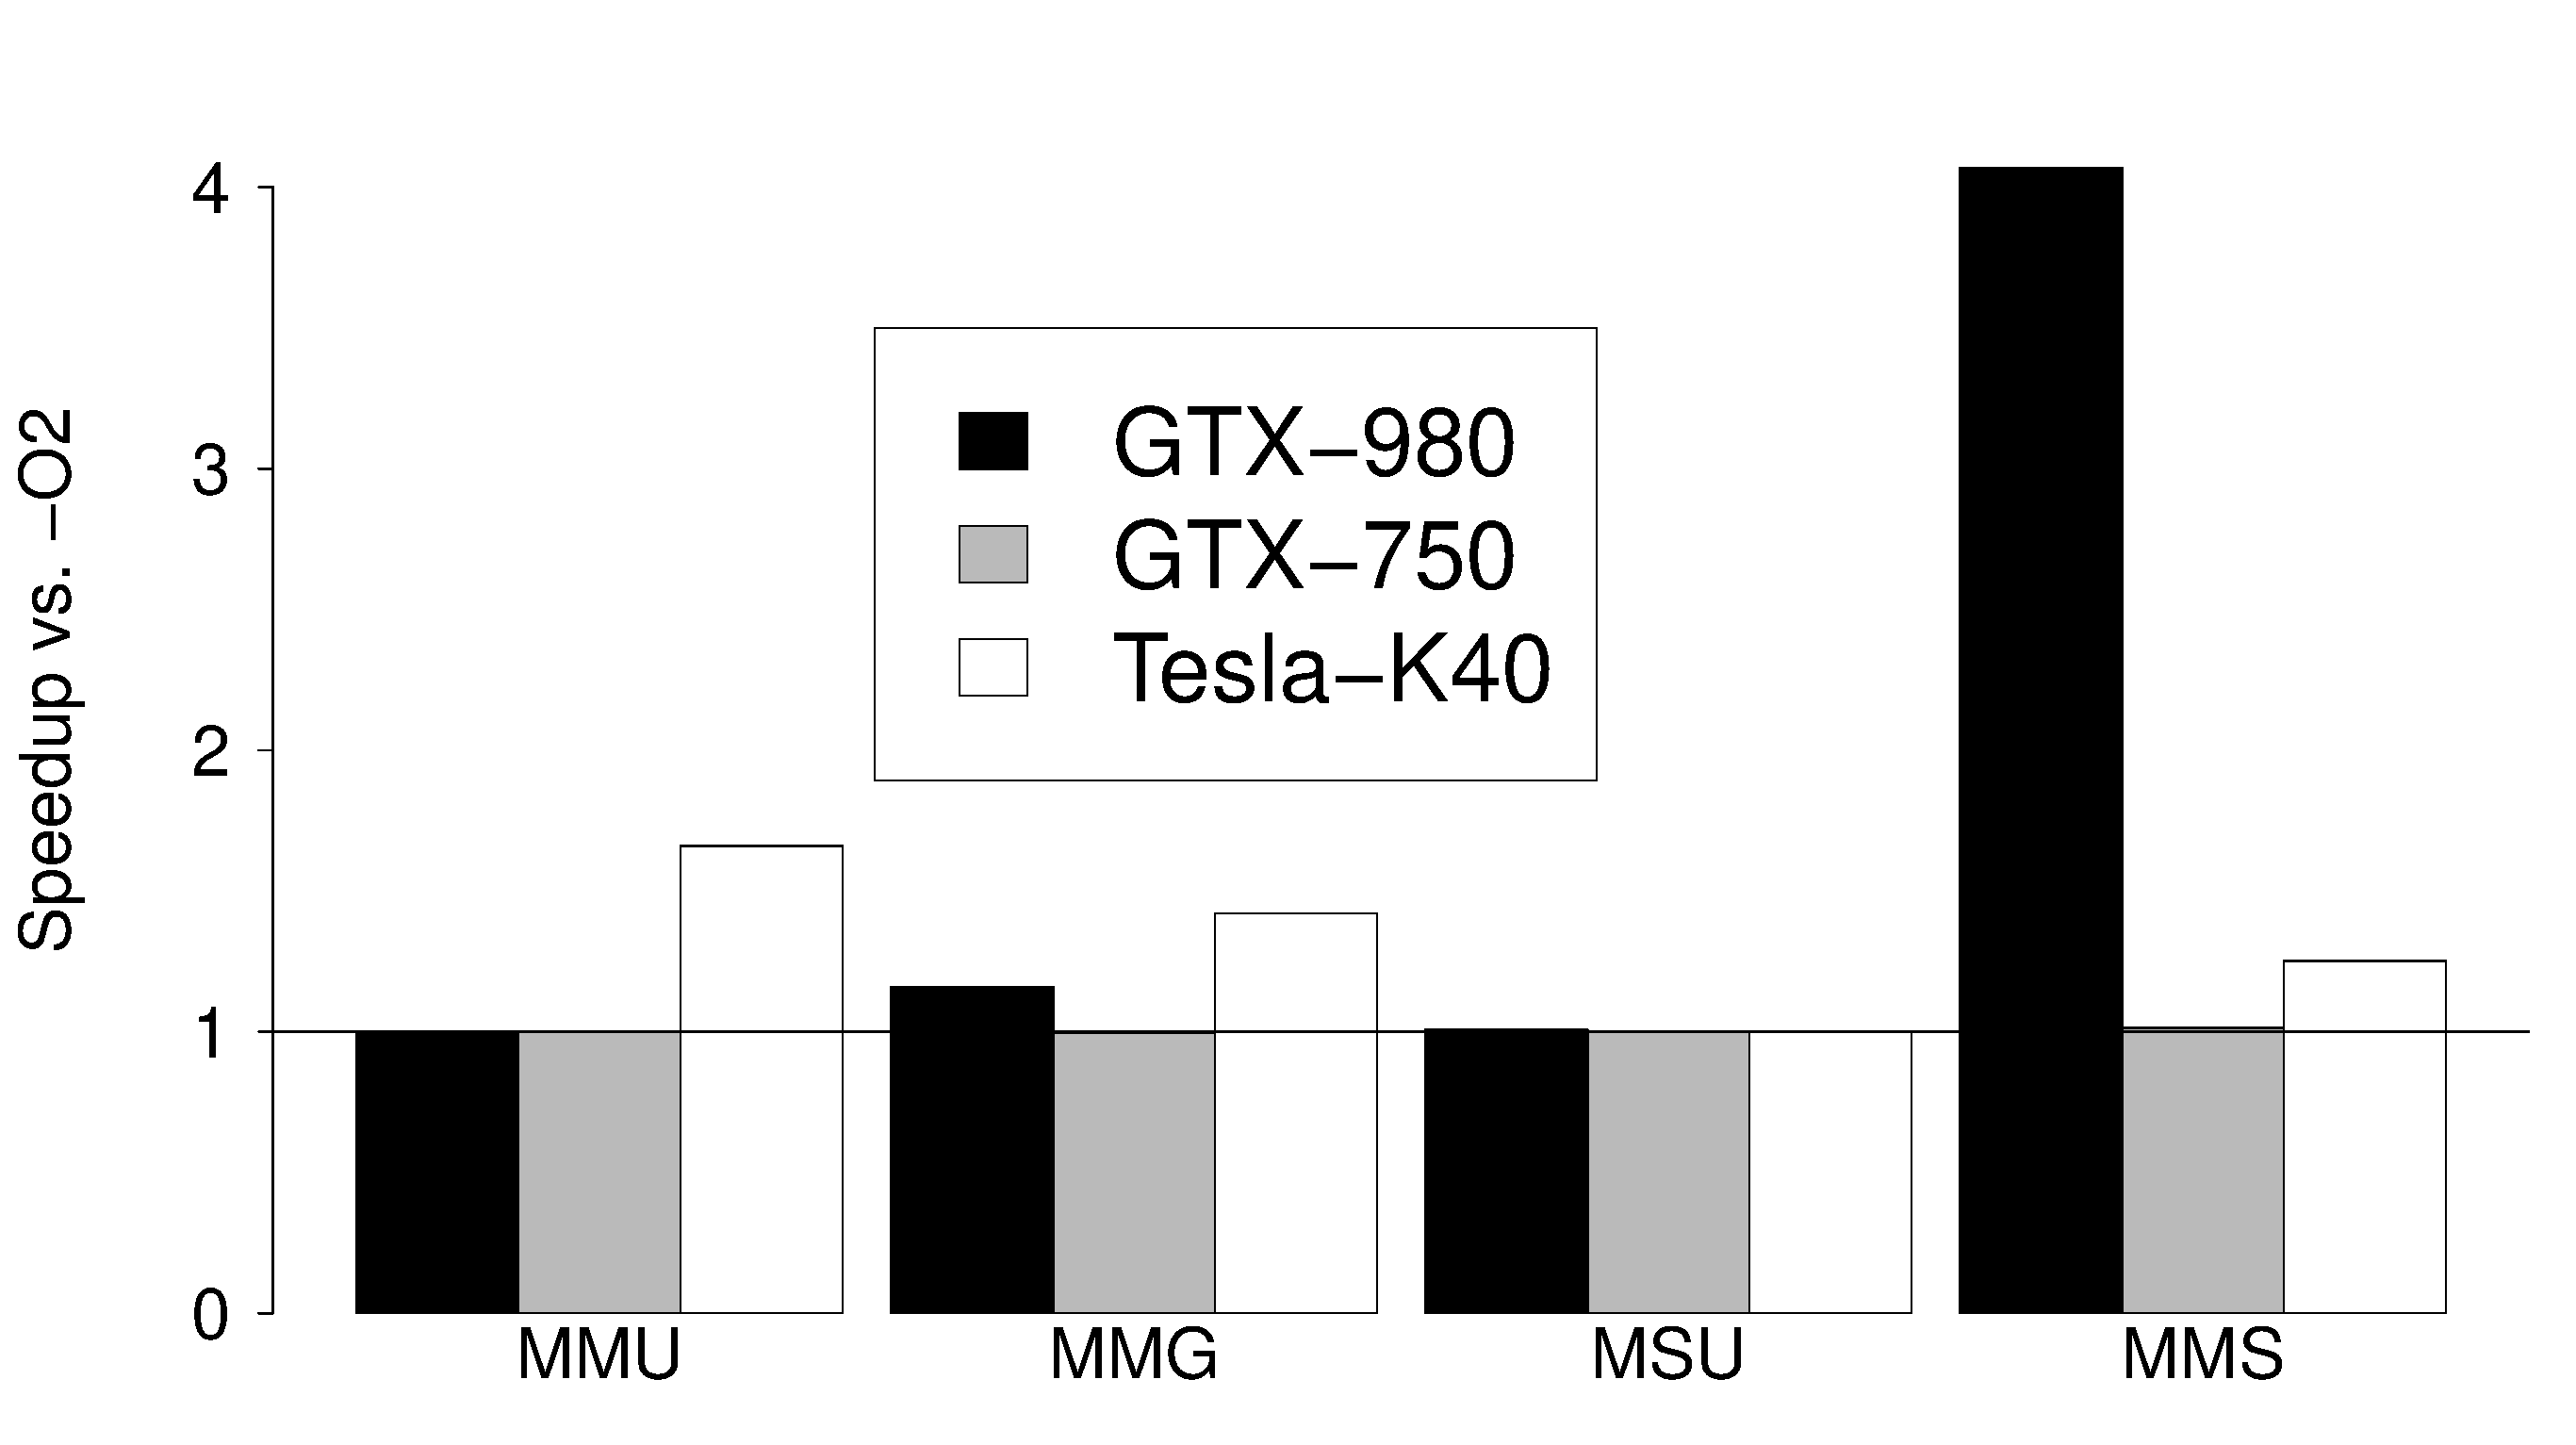
\includegraphics[scale=.2]{images/MatrixSummary.eps}
    \caption{Summary of the speedups achieved versus \emph{-O2} in matrix multiplication versions}
    \label{fig:autotuning}
\end{figure}

% \subsection{Concurrent Streams on GPU}\label{sec:StreamGPU}
Heterogeneous computing is about efficiently using all processors in the system, including CPUs and GPUs.  In our heterogeneous systems, GPUs have been connected to a host machine by a high bandwidth interconnect such as PCI Express (PCIe). Host and device have different memory address spaces, and data must be copied back and forth between the two memory pools explicitly by the data transfer functions. 
%There are two main aspects to consider when attempting to run an application on both CPUs and GPUs concurrently, namely the communication costs incurred by CPU-GPU communications, and how to efficiently overlap computation and data transfers to reduce said cost.
%On integrated CPU/GPU architectures, ~\cite{Zhang17} suggested that the architecture differences between CPUs and GPUs, as well as limited shared memory bandwidth, are two main factors affecting co-running performance. 
%On SMP systems connected to GPU architectures, beside architectural differences, communications between CPUs and GPUs are another important factor. 
Servers with multi-cores and multi-accelerator devices are primarily connected by PCI-Express (PCIe) bus. GPUs and CPUs are bridged by a PCIe bus. Data are copied from the CPU host memory to PCIe memory first, and are then transferred to the GPU's global memory. The PCIe bandwidth is always a crucial performance bottleneck to be improved. 

Congestion control mechanisms have a significant impact on communications. Moreover, the PCIe congestion behavior varies significantly depending on the conflicts created by communication. \cite{Martinasso16} have explored the impact of PCIe topology, which is one major parameter influencing the available bandwidth. They developed a congestion-aware performance model for PCIe communication. They found that bandwidth distribution behavior is sensitive to the transfer message size. PCIe congestion can be hidden if the overlapping communications transfer very small message sizes. However, when the message size reaches some limit, congestion will significantly reduce the theoretical transfer bandwidth efficiency and the bandwidth between the CPU host memory and the GPU memory is far less than PCIe bandwidth. Nvidia provides ways to pin memory, also called paged-locked memory~\citep{CUDAGuide}. A pinned page can be remapped to a PCIe buffer to eliminate data transfer between the host memory and the PCIe buffer. However, consuming too much page-locked memory will reduces overall system performance.

CUDA's programming model provides constructs based on streaming which are capable to schedule multiple kernels concurrently. One CUDA stream can encapsulate multiple kernels, and they have to be scheduled so they strictly follow a particular order. However, kernels from multiple streams can be scheduled to run concurrently. Operations in different streams can be interleaved and overlapped, which can be used to hide data transfers between host and device.

A optimization of GPU applications is to overlap data transfers across the PCIe bus~\citep{Martinasso16}. This is only possible using CUDA streams and pinned memory in the host. Using pinned host memory enables asynchronous memory copies, lowers latency, and increases bandwidth. This way, streams can run concurrently. However, this goal is constrained by the number of kernel engines and copy engines exposed by GPUs, and synchronization must be explicit in the stream kernels. In order to obtain the best performance, a balance between computation and communication needs to be found. If the granularity is too fine, the performance can suffer from the increased communication overhead. On the other side, if the granularity is too coarse or bulk, the performance can suffer from load imbalance. 

There are GPUs with only a single copy engine and a single kernel engine. In this case, data transfer overlapping is not possible. Different streams may execute their commands concurrently or out of order with respect to each other. When an asynchronous CUDA stream is executed without specifying a stream, the CUDA runtime uses the default stream 0; but when a set of independent streams are executed with different ID numbers, these streams avoid serialization, achieving concurrency between kernels and data copies.

Figure~\ref{fig:streams} explains how the streaming model is used to improve the performance of GPU applications. In this figure, we compare the parallel CPU computations of two different GPU version with their respective data transfers: one single stream vs. 3 different kernels with their respective data transfers using 3 streams. The second method is only possible in GPUs with two copy engines, one for host-to-device transfers and another for device-to-host transfers. 


\begin{figure}
	\centering
%     \includegraphics[width=\linewidth]{fig/streams}
    \includegraphics[scale=.8]{images/stream.png}
    \caption{Concurrent Streams overlapping data transfers}
    \label{fig:streams}
%\vspace{-15pt}
\end{figure}








% \subsection{Throughput of Communications and Computation}

% \subsection{Scalability Parameters}






% \section{Runtime and Simulators of Heterogeneous applications}

% \subsection{Simulator GEM5-GPU}

% \subsection{Runtime StarPU + GridSim}

% \subsection{Runtime Darts}


